\chapter{Queue Results}
\label{app:queues}

\vspace{-20pt}
\section{Cache Misses}
\begin{figure}[H]
    \centering
    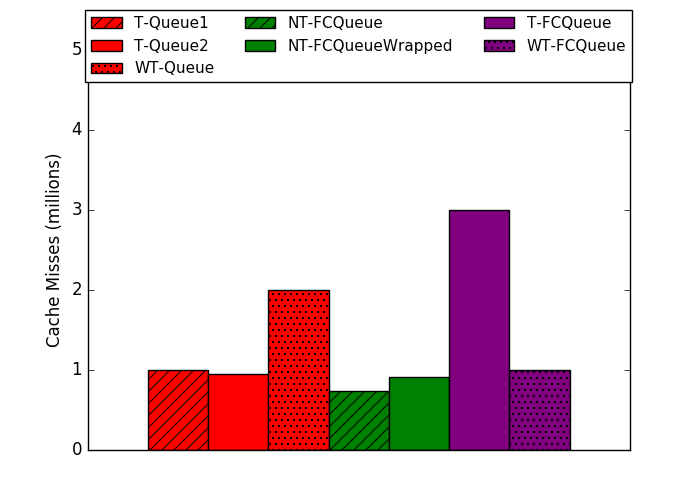
\includegraphics[width=0.66\textwidth]{fcqueues/cm.png}
    \caption{Queue Cache Misses}
    \caption*{
Cache misses are recorded by running the Multi-Thread Singletons Test benchmark with 8 threads, with each thread performing 9M transactions, under the profiling tool Performance Events for Linux (\texttt{perf}). The sampling period is set to 1000, meaning that every 1000th cache miss is recorded.
    In these results, we report the number of cache misses reported by perf (approximately 1/1000 of the actual number of cache misses.)}
\label{fig:qcm}
\end{figure}

\section{Performance of Non-transactional Concurrent Queues}
\begin{figure}[H]
    \centering
    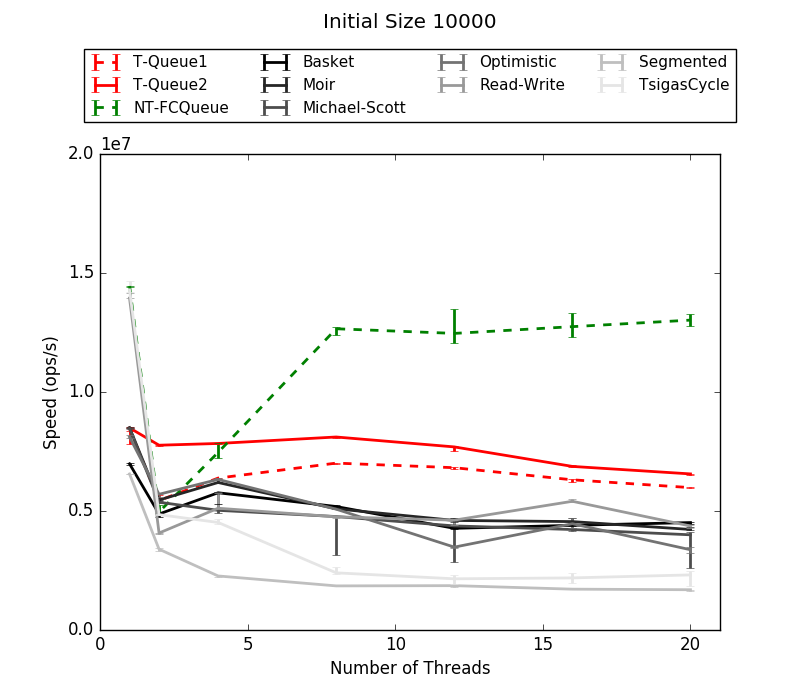
\includegraphics[width=0.65\textwidth]{concurrent/allQ:RandSingleOps10000.png}
    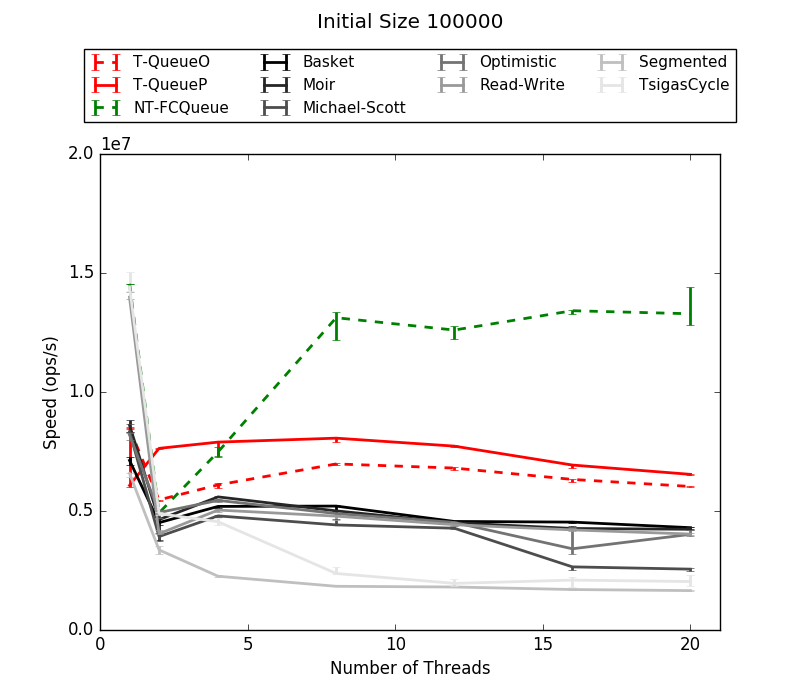
\includegraphics[width=0.65\textwidth]{concurrent/allQ:RandSingleOps100000.png}
    \caption{Non-transactional Queues: Multi-Thread Singletons Test}
\end{figure}
\begin{figure}[H]
    \centering
    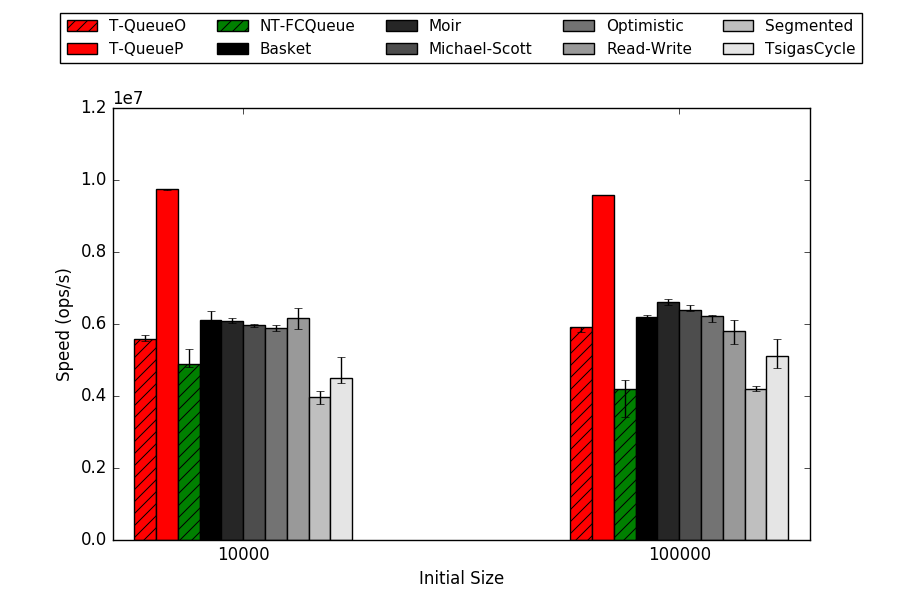
\includegraphics[width=\textwidth]{concurrent/allQ:PushPop.png}
    \caption{Non-transactional Queues: Push-Pop Test}
\end{figure}

\section{Performance of Various Transactional Queues}
\begin{figure}[H]
    \centering
    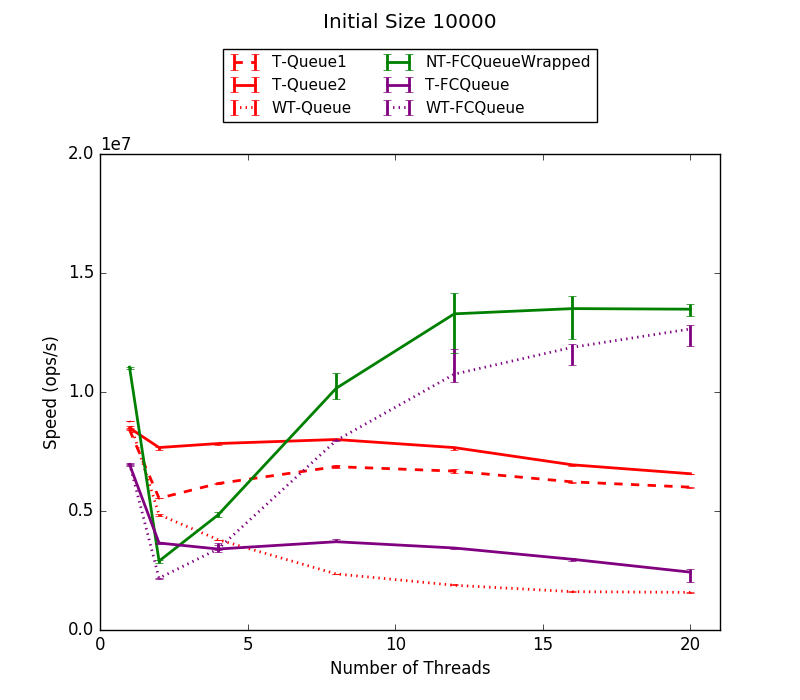
\includegraphics[width=0.85\textwidth]{fcqueues/allQ:RandSingleOps10000.png}
    \vspace{20pt}
    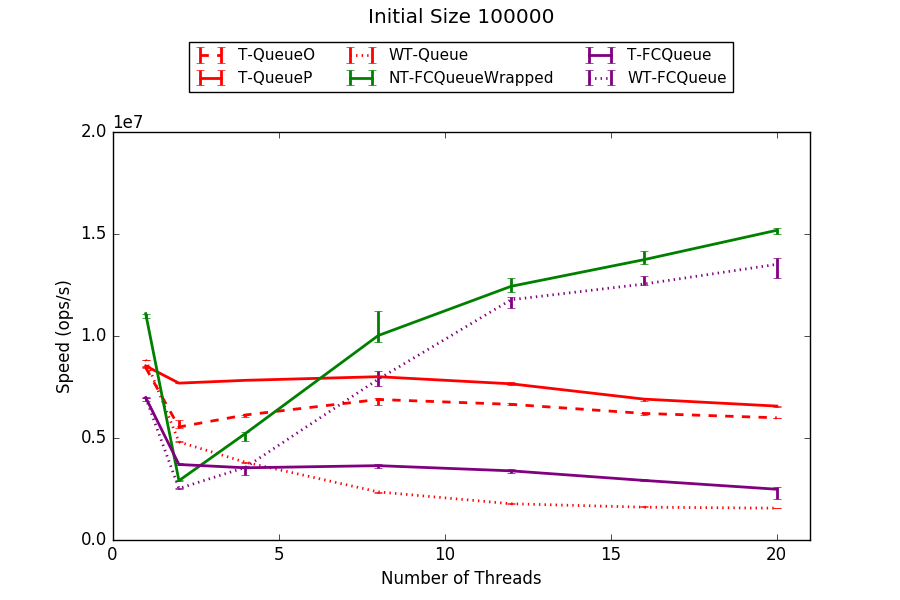
\includegraphics[width=0.85\textwidth]{fcqueues/allQ:RandSingleOps100000.png}
    \caption{Various Transactional Queues: Multi-Thread Singletons Test}
\end{figure}
\begin{figure}[H]
    \centering
    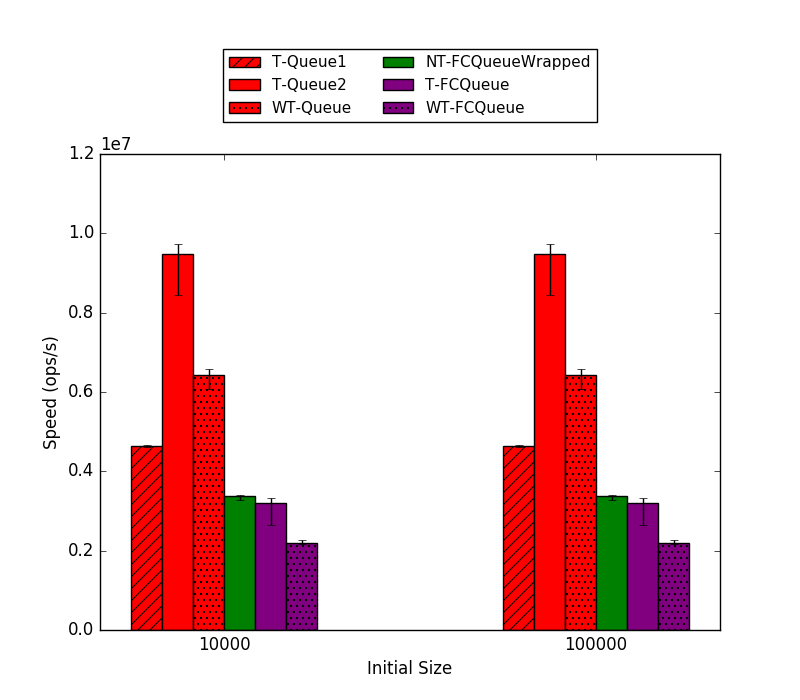
\includegraphics[width=\textwidth]{fcqueues/allQ:PushPop.png}
    \caption{Various Transactional Queues: Push-Pop Test}
\end{figure}

\section{Abort Rate Results}
\label{app:queue_mt}

\begin{table}[H]
\begin{figure}[H]
    \centering
    \begin{tabular}{|c|c|c|}
\hline
\multirow{2}{*}{Queue} & \multicolumn{2}{c|}{Initial Size}\\\cline{2-3}& \qquad 10000 \qquad\quad & \qquad 100000\qquad\quad\\
\hline
\hline
T-QueueO & 0.00001 & 0.00001\\
T-QueueP & 1.54560 & 1.60886\\
T-FCQueue & 0.62494 & 1.62620\\
WT-FCQueue & 0.00000 & 0.00000\\
\hline\end{tabular}

    \caption*{Push-Pop Test}
\end{figure}
\begin{figure}[H]
    \centering
        \begin{tabular}{|c|c|c|c|}
\hline
\multirow{2}{*}{Queue} & \multicolumn{3}{c|}{\#Threads}\\\cline{2-4}& \quad 4 & 12 & 20\\
\hline
\hline
T-QueueO & 10.21210 & 7.46284 & 6.33827\\
T-QueueP & 2.84958 & 2.26892 & 2.32787\\
NT-FCQueueWrapped & 0.00000 & 0.00000 & 0.00000\\
T-FCQueue & 6.08289 & 4.78435 & 5.33221\\
WT-FCQueue & 0.00000 & 0.00000 & 0.00000\\
\hline\end{tabular}

    \caption*{Multi-Thread Singletons Test: Initial Size 10000}
\end{figure}
\begin{figure}[H]
    \centering
    \begin{tabular}{|c|c|c|c|}
\hline
\multirow{2}{*}{Queue} & \multicolumn{3}{c|}{\#Threads Abort Rate (\%)}\\\cline{2-4}& \quad 4 & 12 & 20\\
\hline
\hline
T-Queue1 & 9.405 & 6.841 & 6.303\\
T-Queue2 & 2.809 & 2.324 & 2.446\\
WT-Queue & 16.600 & 59.998 & 71.140\\
NT-FCQueueWrapped & 0.000 & 0.000 & 0.000\\
T-FCQueue & 4.436 & 3.521 & 4.207\\
WT-FCQueue & 0.000 & 0.000 & 0.000\\
\hline\end{tabular}

    \caption*{Multi-Thread Singletons Test: Initial Size 100000}
\end{figure}
    \caption{Queue Test Abort Rate Results}
\end{table}
